%%%%%%%%%%%%%%%%%%%%%%%%%%%%%%%%%%%%%%%%%%%%%%%%%%%%%%%%%%%%%%%%%%%%%%%%%%%%%%%%
% Preambles
%%%%%%%%%%%%%%%%%%%%%%%%%%%%%%%%%%%%%%%%%%%%%%%%%%%%%%%%%%%%%%%%%%%%%%%%%%%%%%%%
\documentclass[aspectratio=169,xcolor=x11names,table]{beamer}
\mode<presentation>{
	% theme
	\usetheme{Luebeck}
	\hypersetup{pdfpagemode=FullScreen}
		\setbeamertemplate{headline}[default]
	\setbeamertemplate{navigation symbols}{}
	% \setbeamertemplate{caption}[numbered]
		\usefonttheme{professionalfonts}
	% logo
	% \addtobeamertemplate{frametitle}{}{
	% 	\begin{textblock*}{100mm}(0.8\textwidth,-7mm)
	% 		
\includegraphics[height=5mm]{sams.jpg}
	% 	\end{textblock*}
	% }
	% footnote
	\setbeamertemplate{footline}[text line]{%
			\parbox{\linewidth}{\vspace*{-8pt}Tutorial - Time Sereies Analysis\hfill\insertshortauthor\hfill\insertframenumber/\inserttotalframenumber}}

	% transparent cover
	\setbeamercovered{transparent}
}

% define your own colors:
\definecolor{KFUPMgreen}{cmyk}{0.756,0,0.756,0.196}
\definecolor{tech_gold}{RGB}{179,163,105}
\definecolor{buzz_gold}{RGB}{234,170,0}
\definecolor{tech_blue}{RGB}{0,38,58}
\definecolor{sams_dark_blue}{RGB}{0,75,141}
\definecolor{sams_medium_blue}{RGB}{0,105,170}
\definecolor{sams_light_blue}{RGB}{0,129,198}
\definecolor{sams_green}{RGB}{93,151,50}
\setbeamercolor{structure}{fg=sams_dark_blue, bg=white}
\setbeamercolor*{palette primary}{use=structure,fg=white,bg=sams_medium_blue}

%%%%%%%%%%%%%%%%%%%%%%%%%%%%%%%%%%%%%%%%%%%%%%%%%%%%%%%%%%%%%%%%%%%%%%%%%%%%%%%%
% Dependencies
%%%%%%%%%%%%%%%%%%%%%%%%%%%%%%%%%%%%%%%%%%%%%%%%%%%%%%%%%%%%%%%%%%%%%%%%%%%%%%%%
\usepackage[utf8]{inputenc}
\usepackage[english]{babel}
\usepackage[backend=bibtex,
	 sorting=none,
	 maxcitenames=2,
	 mincitenames=1,
	 citestyle=authoryear,
	 maxbibnames=99]{biblatex}
\usepackage{csquotes}
\usepackage{lmodern}    % font at arbitrary size
\usepackage{mathtools}
\usepackage{graphicx}
\graphicspath{{fig/}}
\usepackage{color}
\usepackage{bm}
\usepackage{booktabs}
\usepackage{subcaption}
\usepackage{appendixnumberbeamer}
\usepackage{textpos}
\usepackage{datetime}
\usepackage[linesnumbered,ruled,vlined,slovak]{algorithm2e}
\usepackage{animate}
\usepackage{subcaption}
\usepackage{multirow}

%%%%%%%%%%%%%%%%%%%%%%%%%%%%%%%%%%%%%%%%%%%%%%%%%%%%%%%%%%%%%%%%%%%%%%%%%%%%%%%%
% Bibliography
%%%%%%%%%%%%%%%%%%%%%%%%%%%%%%%%%%%%%%%%%%%%%%%%%%%%%%%%%%%%%%%%%%%%%%%%%%%%%%%%
\bibliography{time_series.bib}

%%%%%%%%%%%%%%%%%%%%%%%%%%%%%%%%%%%%%%%%%%%%%%%%%%%%%%%%%%%%%%%%%%%%%%%%%%%%%%%%
% Title Page
%%%%%%%%%%%%%%%%%%%%%%%%%%%%%%%%%%%%%%%%%%%%%%%%%%%%%%%%%%%%%%%%%%%%%%%%%%%%%%%%
\title{Robust Time Series Analysis and Applications}
\subtitle{An Industry Perspective}
\author[Lijun Zhu]{
	{\Large Lijun Zhu}\\
	\vspace{3mm}
	Senior Manager
}
\institute{Data Science and Engineering, Sam's Club}
\newdate{date}{17}{11}{2022}
\date{\small\displaydate{date}}

%%%%%%%%%%%%%%%%%%%%%%%%%%%%%%%%%%%%%%%%%%%%%%%%%%%%%%%%%%%%%%%%%%%%%%%%%%%%%%%%
%  Outline at each section
%%%%%%%%%%%%%%%%%%%%%%%%%%%%%%%%%%%%%%%%%%%%%%%%%%%%%%%%%%%%%%%%%%%%%%%%%%%%%%%%
\AtBeginSection[] {
    \begin{frame}
        \frametitle{Outline}
        \tableofcontents
        [
            currentsection,
            currentsubsection,
            subsectionstyle=show/show/hide
        ]
        \addtocounter{framenumber}{-1}
    \end{frame}
}

%%%%%%%%%%%%%%%%%%%%%%%%%%%%%%%%%%%%%%%%%%%%%%%%%%%%%%%%%%%%%%%%%%%%%%%%%%%%%%%%
% Content
%%%%%%%%%%%%%%%%%%%%%%%%%%%%%%%%%%%%%%%%%%%%%%%%%%%%%%%%%%%%%%%%%%%%%%%%%%%%%%%%
\begin{document}

% title page
{
	%
	\usebackgroundtemplate{
\includegraphics[width=1\paperwidth]{sams_background}}
	%
	\begin{frame}[noframenumbering,plain]
		% \hfill
		% \begin{minipage}{0.65\paperwidth}
		\titlepage
		% \end{minipage}
	\end{frame}
	\setcounter{framenumber}{0}
}

% introduction
\begin{frame}{Who am I?}
	\begin{columns}
		\begin{column}{0.8\linewidth}
		\begin{itemize}
			\item Lijun Zhu, Ph.D.
				\begin{itemize}
					\item Machine Learning, Data Science, and Signal Processing
					\item Leading a team of 10-20 DS, DE, MLE, and SWE
					\item Previous experience in internship, Co-op, IC, and PM
				\end{itemize}
			\item Sam's Club Data Science and Engineering
				\begin{itemize}
					\item A centralized data science / machine learning group
					\item Full stack data scientists from product concept to production
					\item Impactful product and initiatives spanning all field in data science
						\begin{itemize}
							\item Time series forecast
							\item Optimization
							\item NLP chat bot and text analysis
							\item Fraud detection
						\end{itemize}
				\end{itemize}
			\item Full time and internship opportunities every year
				\begin{itemize}
					\item Organization trippled in size for the past three years
				\end{itemize}
		\end{itemize}
		\end{column}
		\hfill
		\begin{column}{0.2\linewidth}
			\begin{figure}
				\centering
				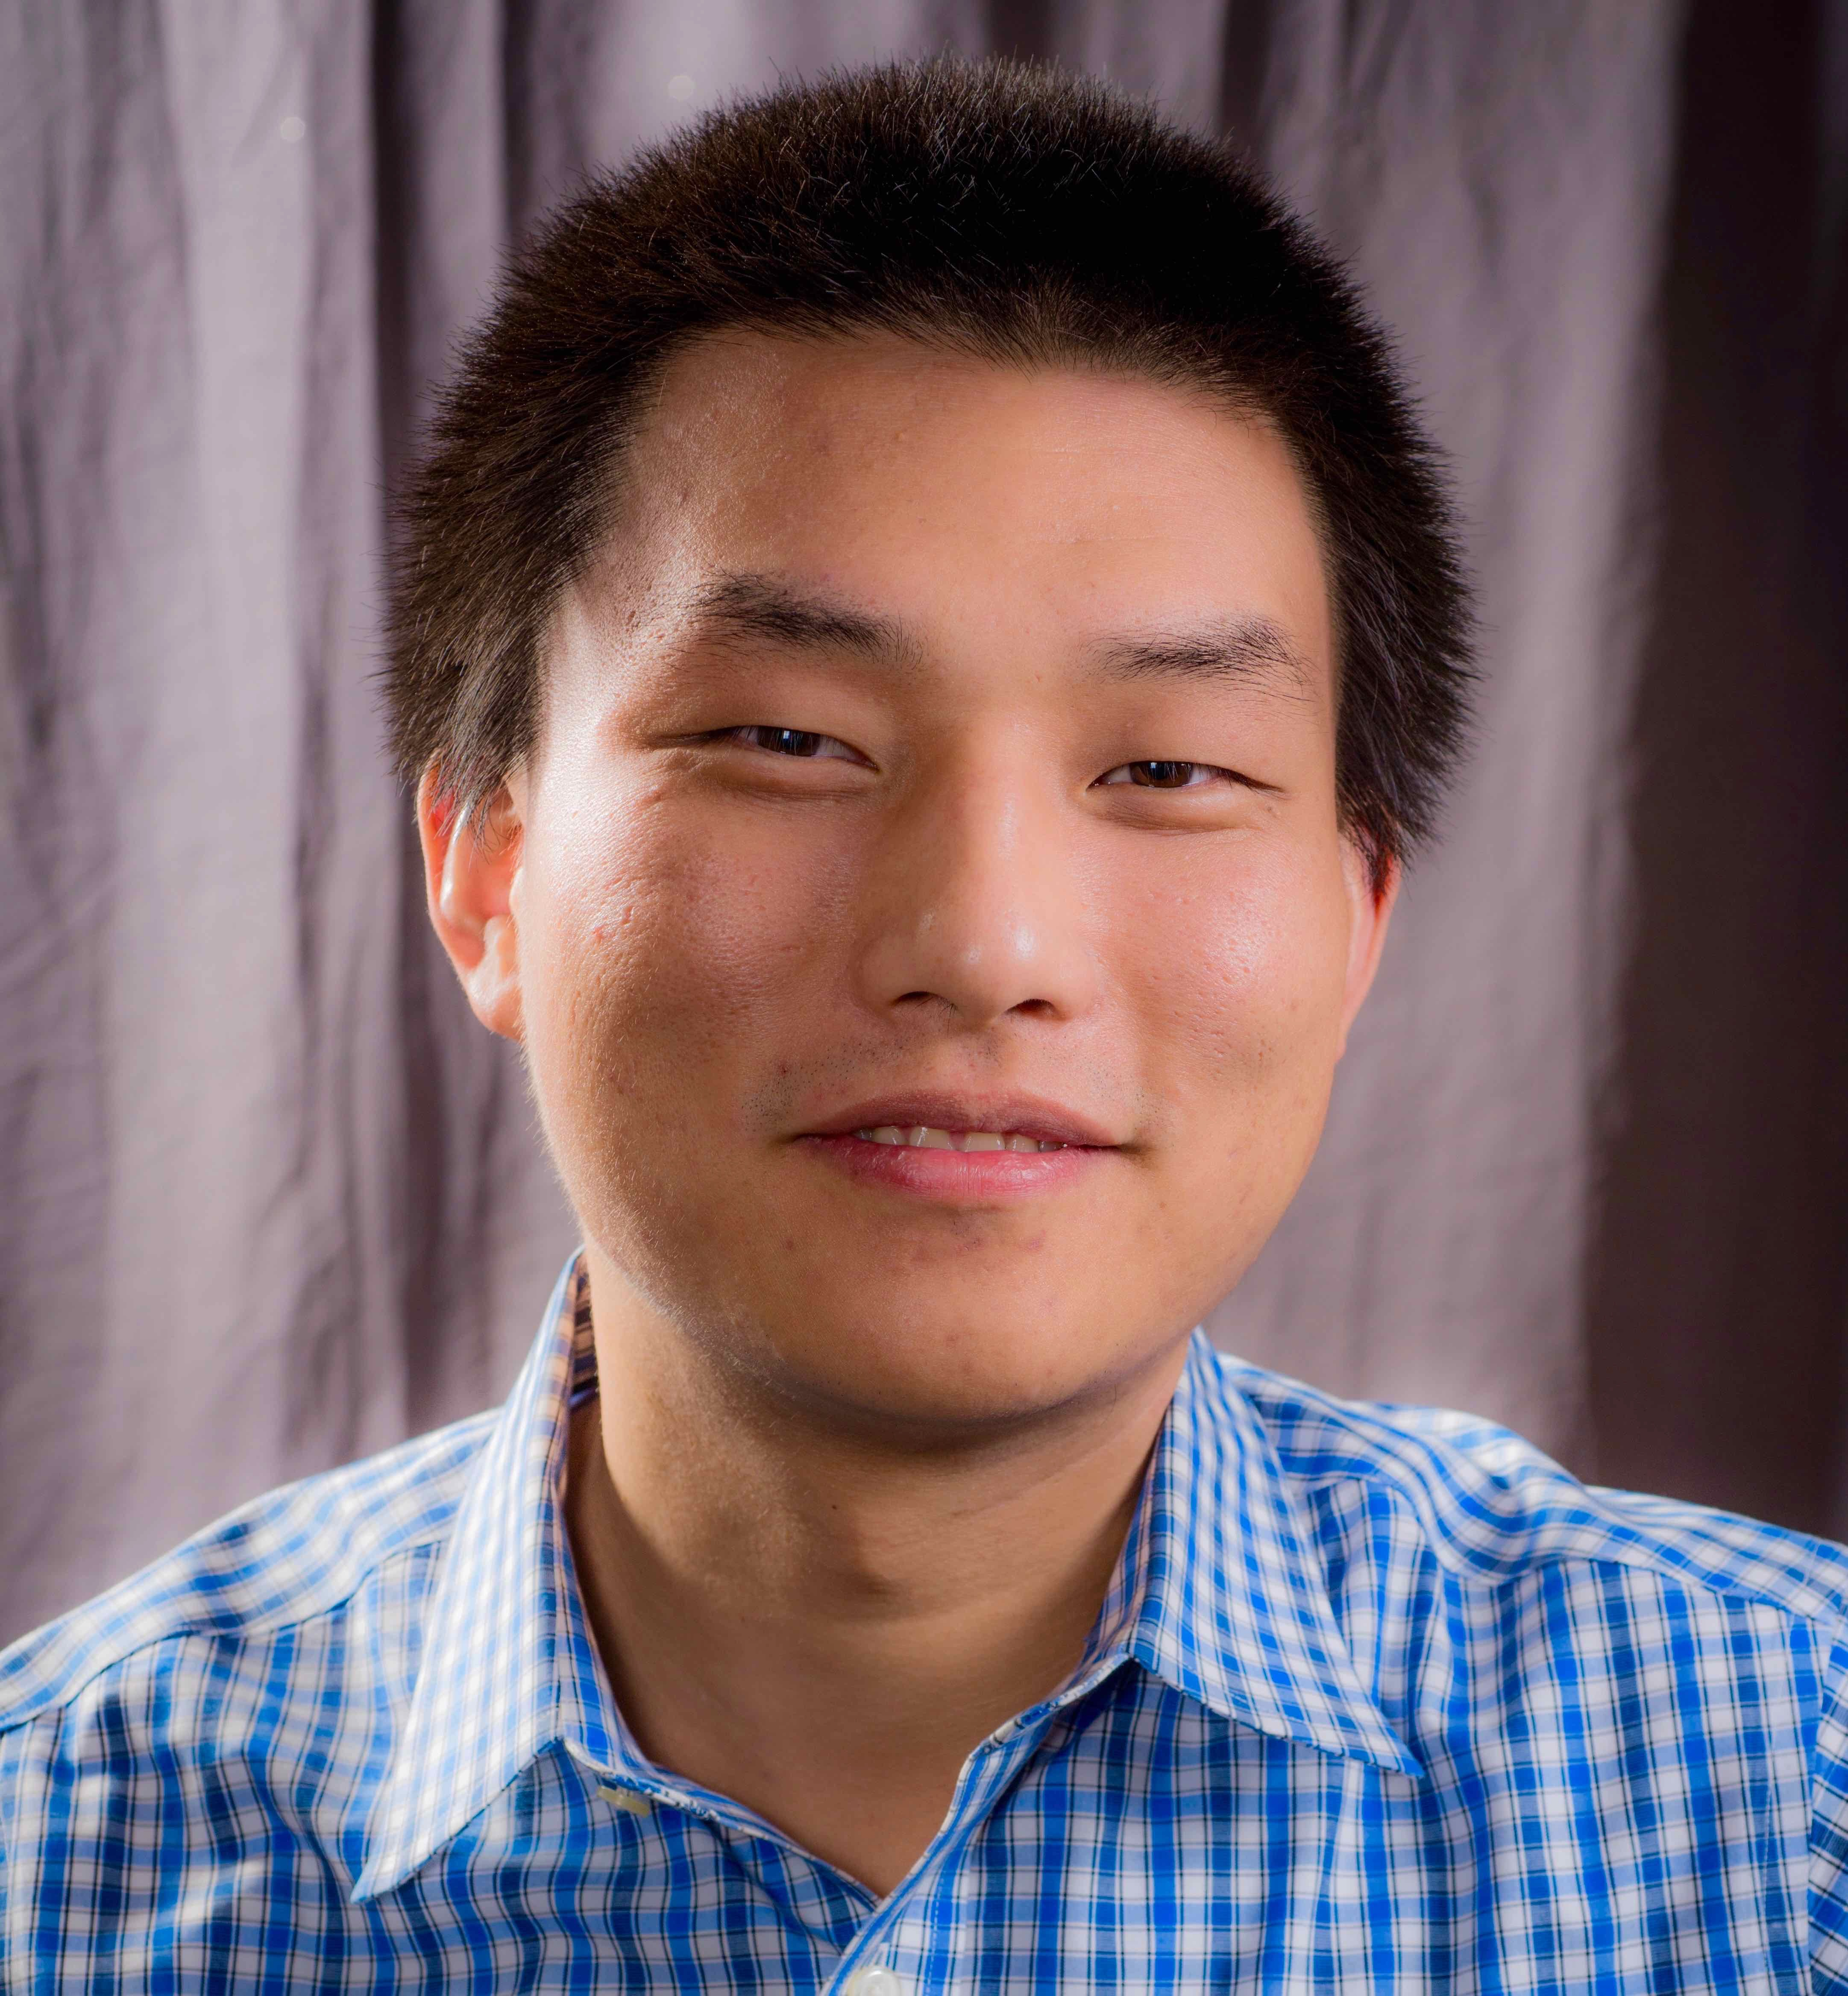
\includegraphics[width=\columnwidth]{lijun}
			\end{figure}
			\vspace{2mm}
			\begin{figure}
				\centering
				
\includegraphics[width=\columnwidth]{sams_logo}
			\end{figure}
		\end{column}
	\end{columns}
\end{frame}

\begin{frame}
	\frametitle{Outline}
	\tableofcontents[hideallsubsections]
\end{frame}

%-------------------------------------------------------------------------------
% Time series analysis basics
%-------------------------------------------------------------------------------
\section{Time series analysis}
\subsection{What is time series}
\begin{frame}
	\frametitle{Time Series is Ubiquitous}
	\begin{columns}
		\begin{column}{0.4\linewidth}
			\begin{itemize}
				\item Time series record a history of states
					\begin{itemize}
						\item price hisory
						\item sales records
						\item sensor signal
						\item operational log
					\end{itemize}
				\item History is useful if it helps us make decisions
				\item Decision leads to business impact
			\end{itemize}
		\end{column}
		\hfill
		\begin{column}{0.6\linewidth}
			\begin{figure}
				\centering
				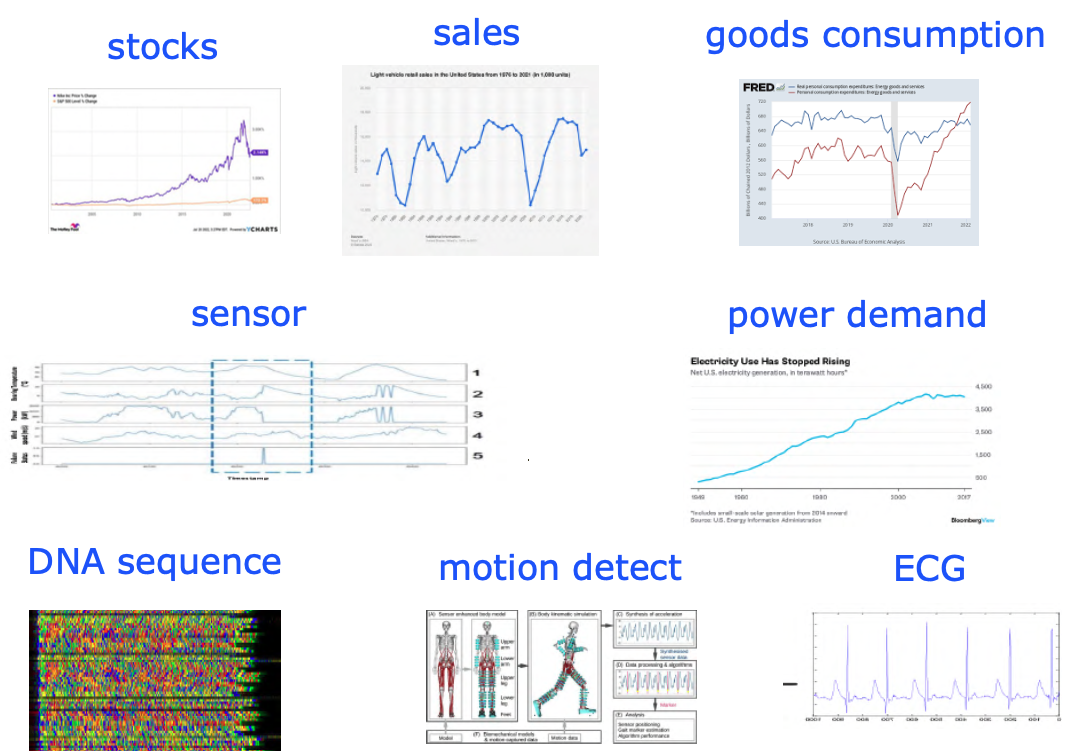
\includegraphics[width=\columnwidth]{time_series}
				\tiny{Image courtesy of \cite{wen2022robust}.}
			\end{figure}
		\end{column}
	\end{columns}
\end{frame}

\begin{frame}
	\frametitle{Typical Applications on Time Series}
	\begin{figure}
		\centering
		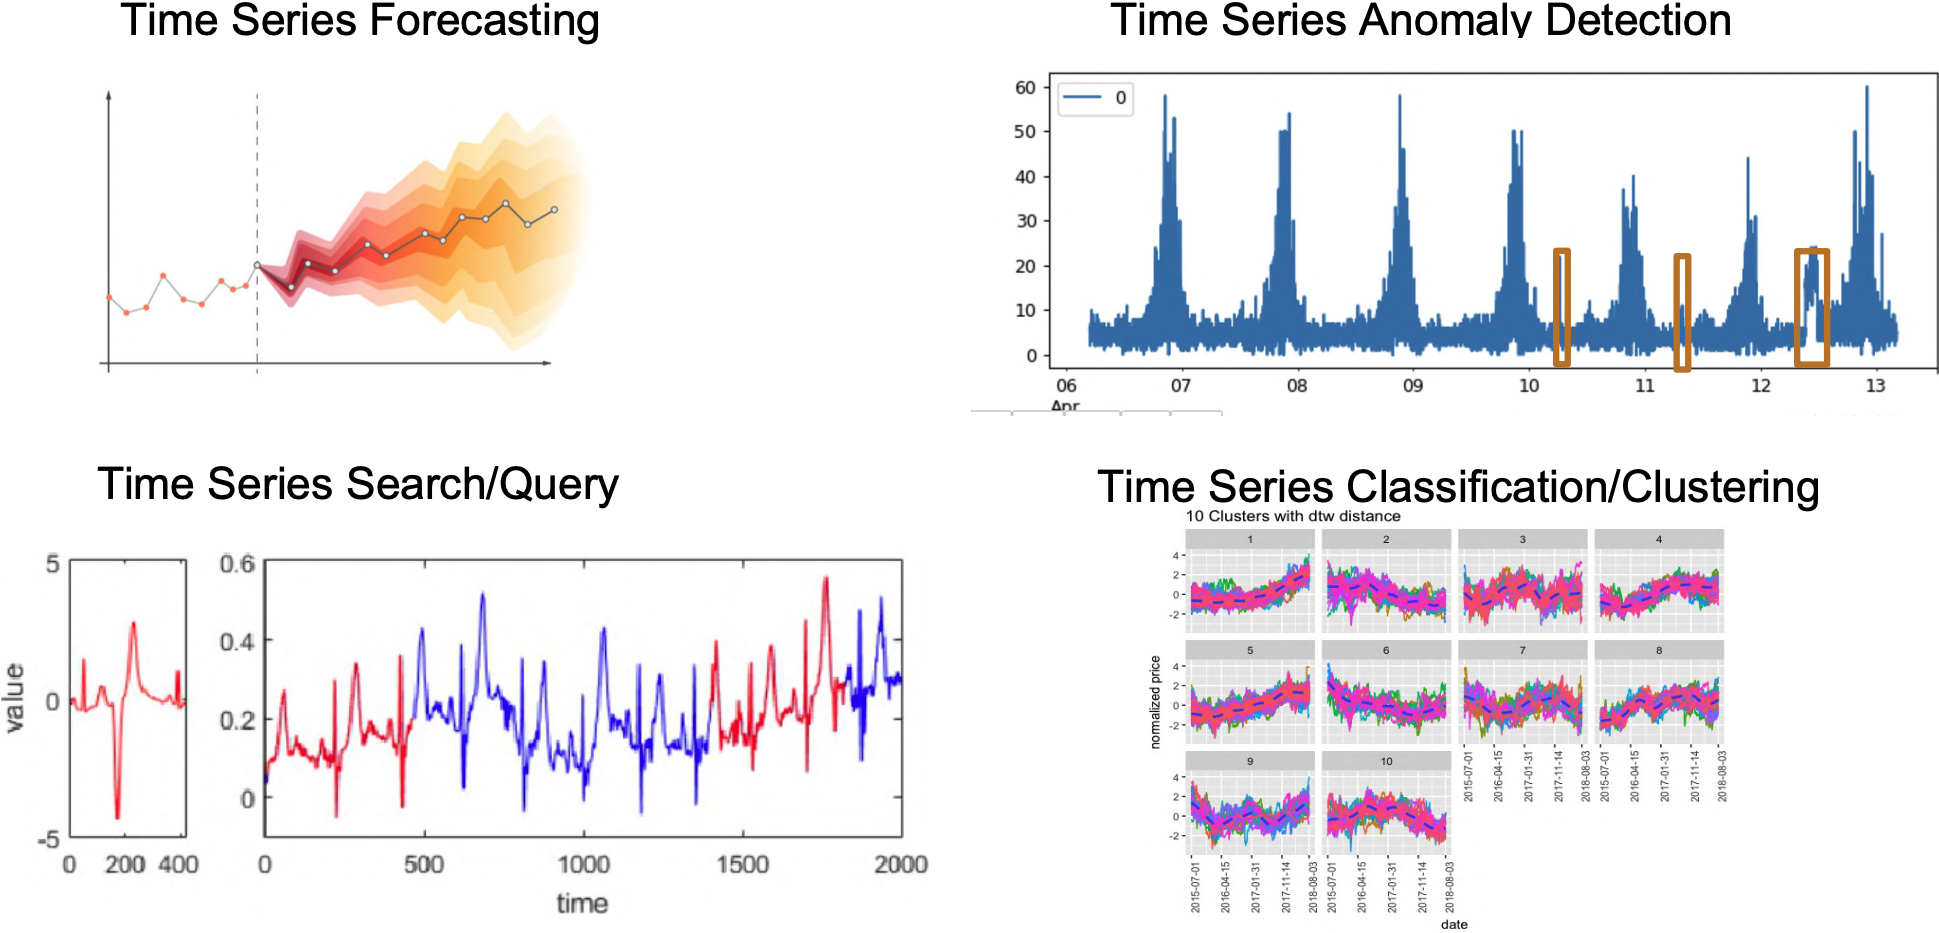
\includegraphics[width=\linewidth]{time_series_applications}
		\tiny{Image courtesy of \cite{wen2022robust}.}
	\end{figure}
\end{frame}

\begin{frame}
	\frametitle{From Forecast to Decision}
	\begin{itemize}
		\item Allocate resource based on demand forecast
		\item Peak demand vs. average demand
		\item Lead time and forecast horizon
	\end{itemize}
	\vfill
	\begin{figure}
		\centering
		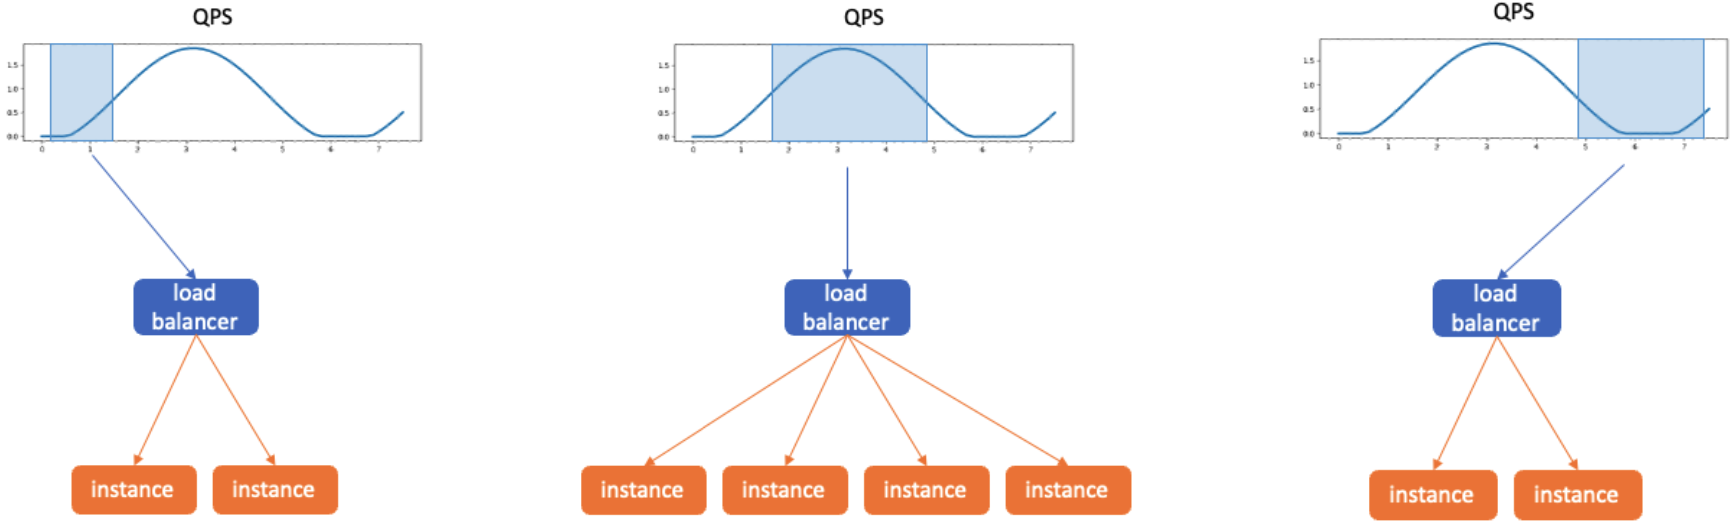
\includegraphics[width=\linewidth]{forecast}
		\tiny{Image courtesy of \cite{wen2022robust}.}
	\end{figure}
\end{frame}

\begin{frame}
	\frametitle{From Anomaly Detection to Cause Analysis}
	\begin{columns}
		\begin{column}{0.4\linewidth}
			\begin{figure}
				\centering
				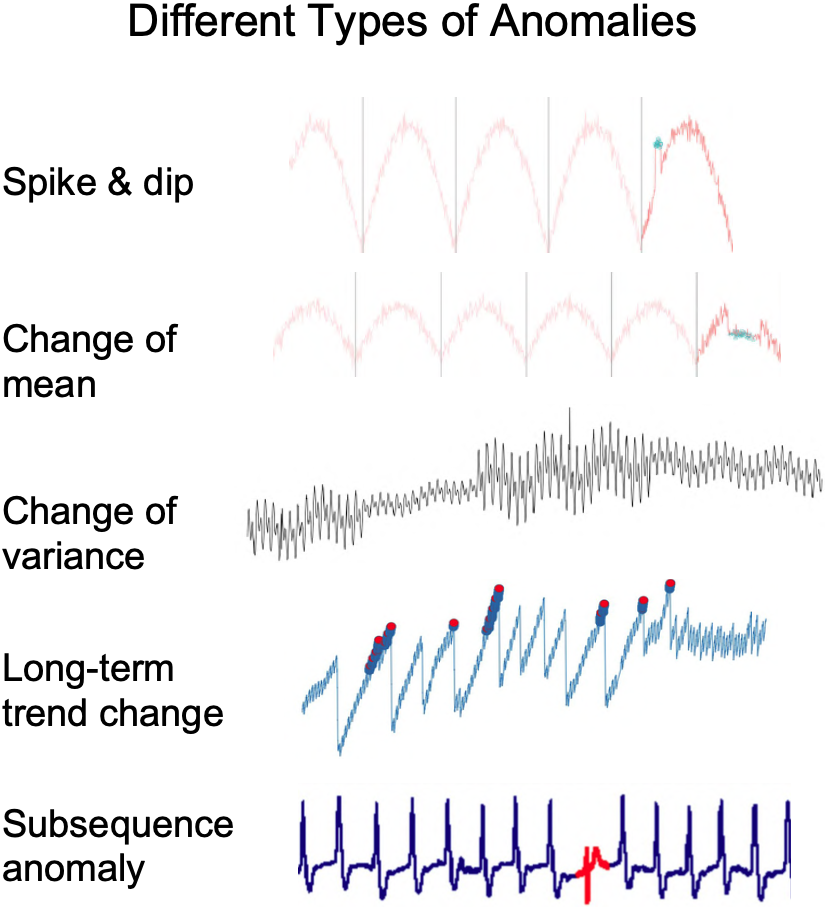
\includegraphics[width=\columnwidth]{anomaly}
			\end{figure}
		\end{column}
		\hfill
		\begin{column}{0.55\linewidth}
			\begin{itemize}
				\item Time series is predictable since some of its properties are stable, e.g. WSS process
					\begin{itemize}
						\item Period
						\item Mean
						\item Variance
						\item Trend
						\item Distribution
					\end{itemize}
				\item Anomaly are the portion of the signal that breaks the previous pattern
				\item Detection of anomaly is only the first step, the key is the root cause of the anomaly
				\item Cause analysis leads to new understanding and improved procedure 
			\end{itemize}
		\end{column}
	\end{columns}
\end{frame}

%-------------------------------------------------------------------------------

\subsection{Values in time series}
\begin{frame}
	\frametitle{Why Time Series (Data Science) Matters?}
	\large
	\begin{itemize}
		\item Data science starts from understanding of observations of physical world / human behaviors
		\vspace{2mm}
		\item The impact of these changes (good or bad) is the value of the data science
			\begin{itemize}
				\item Improved understanding 
				\item Make decision and change procedures
				\item Change future world and behaviors
			\end{itemize}
		\vspace{2mm}
		\item Artificial intelligence in data science is a approach to realize impact
			\begin{columns}
				\hspace{13mm}
				\begin{column}{0.5\linewidth}
					\begin{itemize}
						\item signal processing
						\item statistical analysis
					\end{itemize}
				\end{column}
				\hfill
				\begin{column}{0.5\linewidth}
					\begin{itemize}
						\item machine learning
						\item deep learning
					\end{itemize}
				\end{column}
			\end{columns}
		\vspace{2mm}
		\item Only measurble impact is valued in corporative scenario
			\begin{itemize}
				\item Indivual evaluation: bonus, reward, and promotion
				\item Team growth: budget, resource, exposure
			\end{itemize}
	\end{itemize}
\end{frame}

%-------------------------------------------------------------------------------

\subsection{Methods for time series analysis}

\begin{frame}
	\frametitle{Data Preparation}
	
\end{frame}

\begin{frame}
	\frametitle{Feature Engineering}
	
\end{frame}

\begin{frame}
	\frametitle{Modeling and Experiments}
	
\end{frame}

\begin{frame}
	\frametitle{Visualization and Validation}
	
\end{frame}

%-------------------------------------------------------------------------------
% Industry perspective for campus hires
%-------------------------------------------------------------------------------
\section{Industry perspective}
\subsection{Job market demands}
\begin{frame}
	\frametitle{Roles in my group}
	\begin{itemize}
		\item<1> Data Scientists (DS)
			\begin{itemize}
				\item Convert business problem to a data science problem
				\item Feature engineering, model design, system validation
				\item Visualization and communication to business partners
			\end{itemize}
		\item<2> Data Engineers (DE)
			\begin{itemize}
				\item Work with data stakeholder to collect and store data
				\item Clean up dataset and make it available for data science and engineering teams
				\item Build data pipeline to automate regular data update and monitor data drift
			\end{itemize}
		\item<3> Machine Learning Engineers (MLE)
			\begin{itemize}
				\item Build cloud/software infrastructures to support data science products
				\item Improve model effectiveness and efficiency (new models and tools)
				\item Maintain production ready system and long-term support of data science products
			\end{itemize}
		\item<4> Software Development Engineers (SWE)
			\begin{itemize}
				\item Work with business partner to define data science product
				\item Set requirements and acceptance criteria to data science and engineering teams
				\item Communicate data science and engineer teams' success and limitation
			\end{itemize}
	\end{itemize}
\end{frame}

\begin{frame}
	\frametitle{Other related roles}
	\begin{itemize}
		\item<1> Technical Product Managers (TPM)
			\begin{itemize}
				\item Work with business partner to define data science product
				\item Set requirements and acceptance criteria to data science and engineering teams
				\item Communicate data science and engineer teams' success and limitation
			\end{itemize}
			\vspace{5mm}
		\item<2> Data Analytics
			\begin{itemize}
				\item Conduct A/B tests to measure the effectiveness of data science product
				\item Visualization and reporting of efficiency analysis
			\end{itemize}
			\vspace{5mm}
		\item<3> UI/UX desginers
			\begin{itemize}
				\item Work with business team to identify the requirements for user interface
				\item Collaborate with data science team to provide necessary data for the interface
			\end{itemize}
	\end{itemize}
\end{frame}

\begin{frame}
	\frametitle{Data Scientists (DS)}
\end{frame}

\begin{frame}
	\frametitle{Data Engineers (DE)}
\end{frame}

\begin{frame}
	\frametitle{Machine Learning Engineers (MLE)}
\end{frame}

\begin{frame}
	\frametitle{Software Development Engineers (SWE)}
\end{frame}

%-------------------------------------------------------------------------------

\subsection{A product driving perspective}

\begin{frame}
	\frametitle{Product is your best Testimony}
\end{frame}

\begin{frame}
	\frametitle{Product is the driving force behind innovation}
\end{frame}

%-------------------------------------------------------------------------------

\subsection{A growth mindset}

\begin{frame}
	\frametitle{The Manager's Path (\cite{fournier2017manager})}
	\begin{columns}
		\begin{column}{0.7\linewidth}
			\begin{itemize}
				\item Establish your technical competence as an individual contributer (IC)
				\item Avance and try out management as tech lead
				\item People Manager (PM) is not a promotion but a different job
			\end{itemize}
		\end{column}
		\hfill
		\begin{column}{0.3\linewidth}
			\begin{figure}
				\centering
				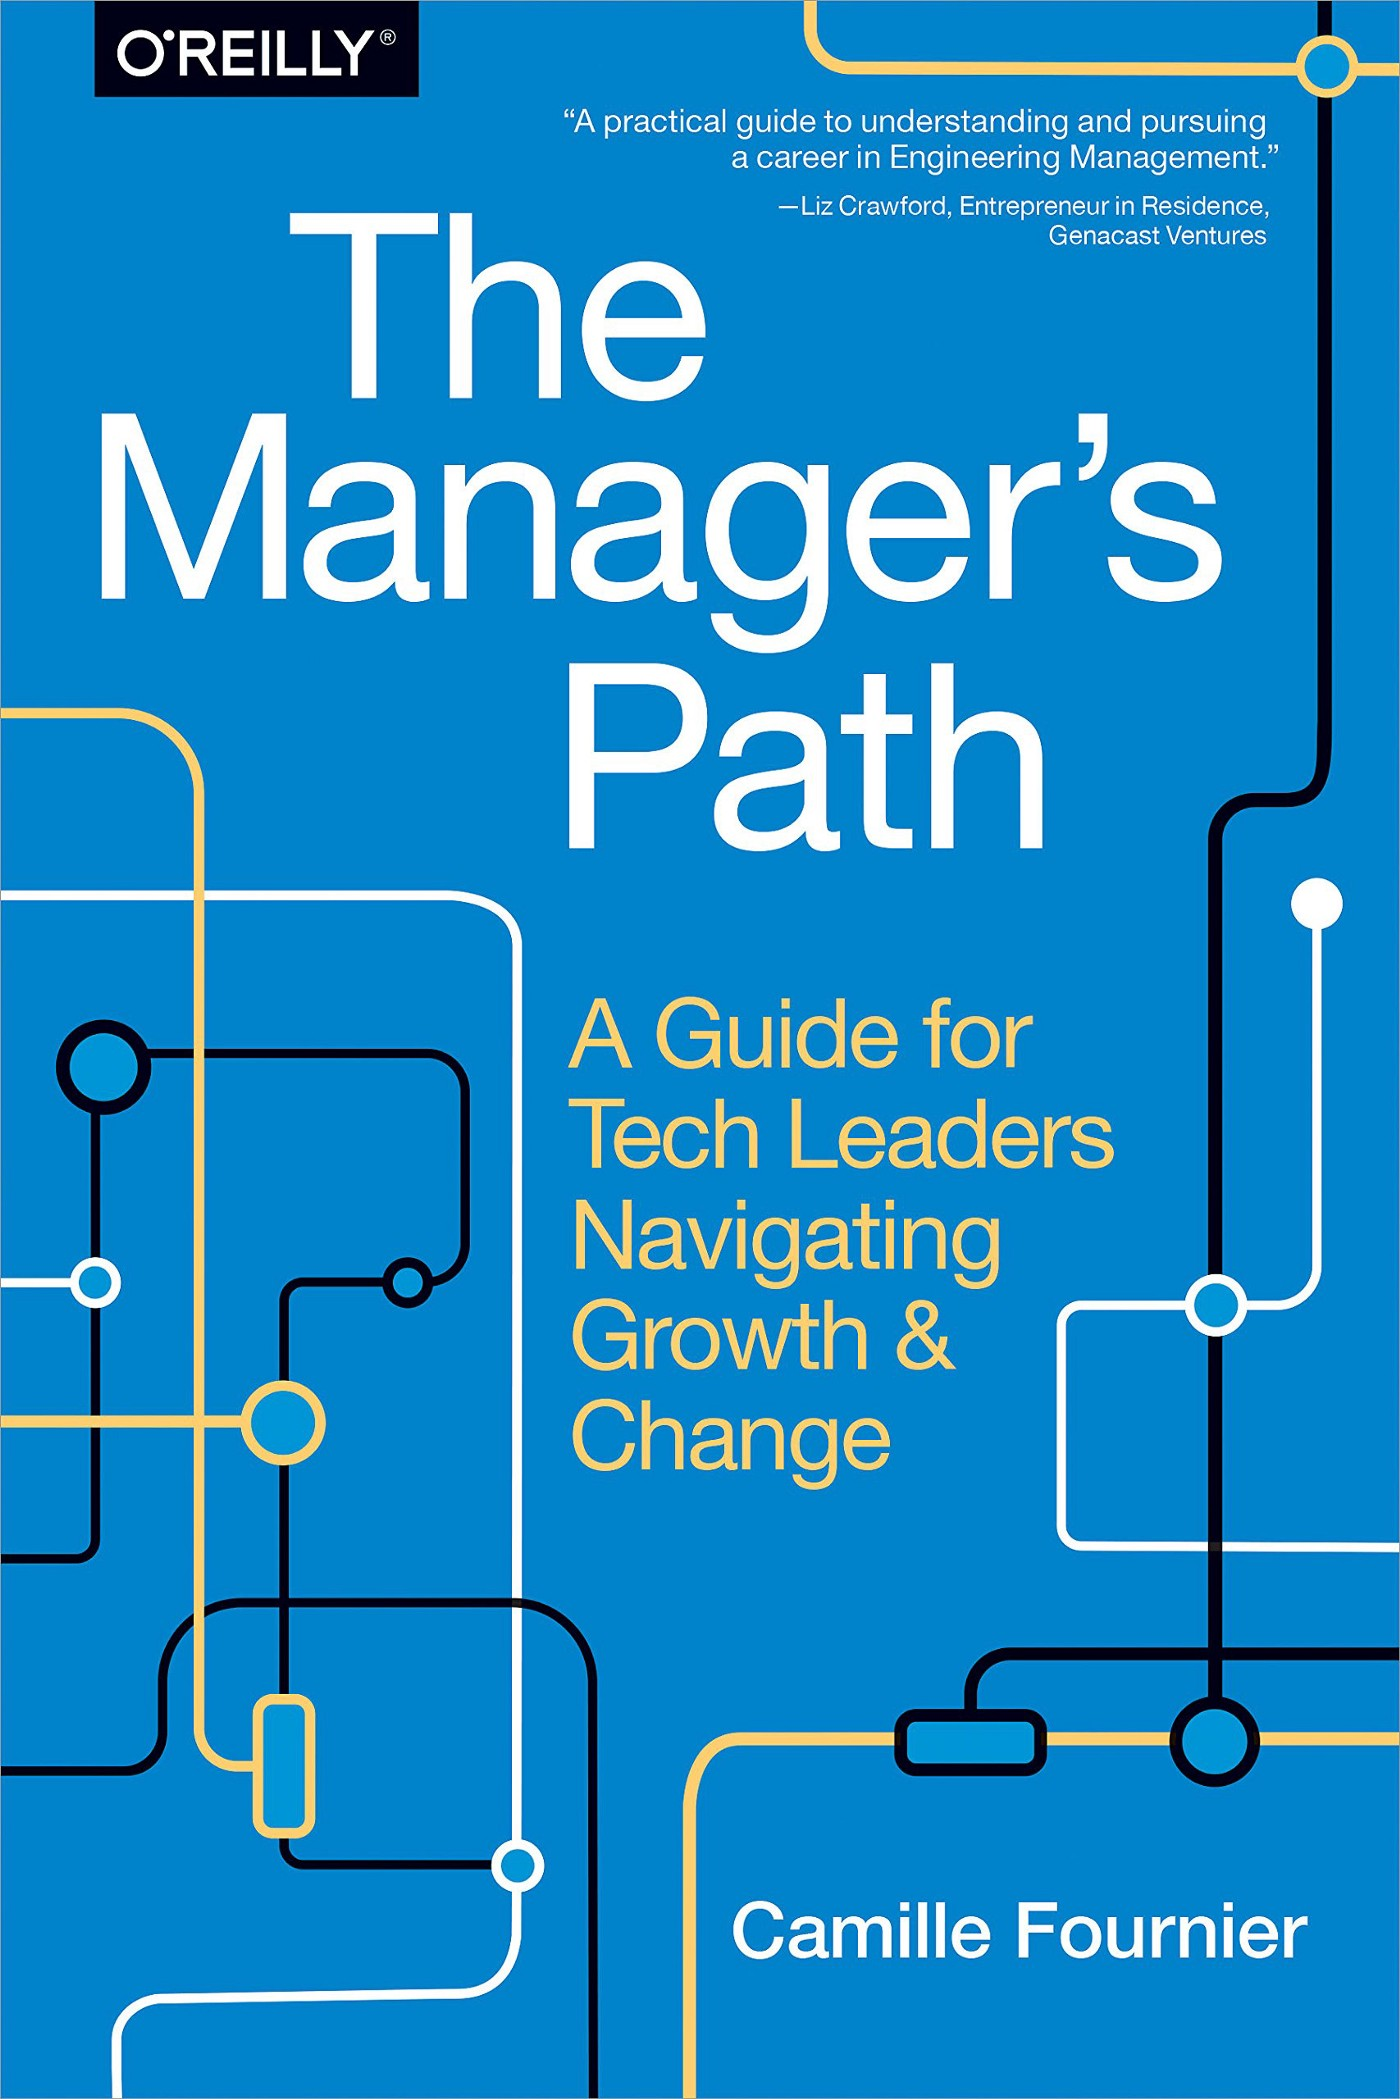
\includegraphics[width=\columnwidth]{manager}
			\end{figure}
		\end{column}
	\end{columns}
\end{frame}

\begin{frame}
	\frametitle{Zero to One (\cite{thiel2014zero})}
	\begin{columns}
		\begin{column}{0.7\linewidth}
			\begin{itemize}
				\item In the long run, innovation is the most important driving force behind economies
				\item Today's best practice leads to dead ends
					\begin{itemize}
						\item You need to be different to be better (Bose)
						\item Fail and fail fast (MSR)
					\end{itemize}
				\item Find values in unexpected places
					\begin{itemize}
						\item Thinking about first principles instead of formulas
						\item Nothing worth learning can be taught
					\end{itemize}
			\end{itemize}
		\end{column}
		\hfill
		\begin{column}{0.3\linewidth}
			\begin{figure}
				\centering
				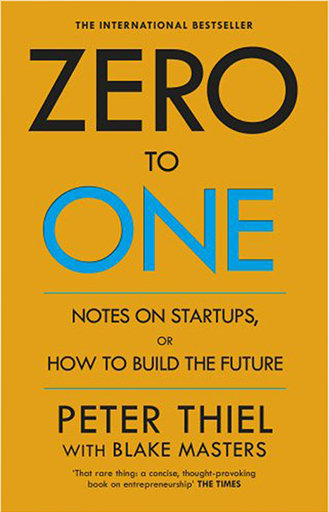
\includegraphics[width=\columnwidth]{zero}
			\end{figure}
		\end{column}
	\end{columns}
\end{frame}

%-------------------------------------------------------------------------------
% Summary
%-------------------------------------------------------------------------------

\begin{frame}
	\frametitle{Summary}
	\tableofcontents
\end{frame}

%-------------------------------------------------------------------------------
% Q & A
%-------------------------------------------------------------------------------
\begin{frame}
	\center
	\Huge Q \& A
\end{frame}

\begin{frame}[t,allowframebreaks]
	\frametitle{References}
	\tiny
	\printbibliography
\end{frame}

\end{document}
